\documentclass{beamer}
\usepackage[utf8]{inputenc}
\usepackage[autostyle]{csquotes}
\usepackage{fancybox}
\usepackage{graphicx}
\usepackage{hyperref}
\usepackage{tabulary}
\usepackage{tabularx}
\usepackage[export]{adjustbox}
 
 
\title{Yubikey}
\author{judge}
\date{20.12.2018}

\usetheme{metropolis}
\usecolortheme{default}

\begin{document}
 
\frame{\titlepage}

%\section{One Key to rule them all}

\begin{frame}
\frametitle{Hardware Security Token}
	\begin{itemize}
		\item{Do Crypto stuff external device}
		\item{No need for multiple keys or copying of keys to different machines}
		\item{There are many Hardware Security tokens, yubikey is a nice low cost variant}
	\end{itemize}
\end{frame}

\begin{frame}
\frametitle{One Key to rule them all}
	\begin{figure}[h]
		\center
		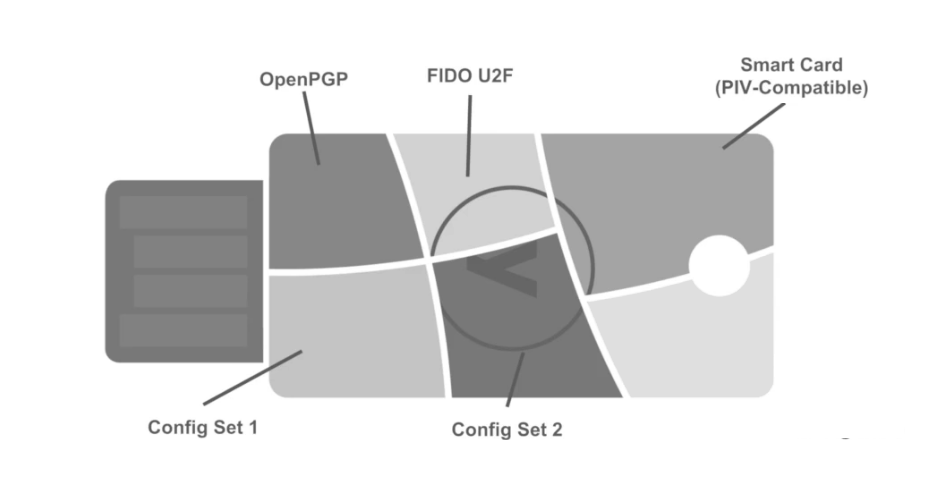
\includegraphics[width=0.7\textwidth]{images/functionality.png}
	\end{figure}
	\begin{columns}
		\column{0.33\textwidth}
			\textbf{Config Slots}
			\begin{itemize}
				\item{symmetric encryption}
				\item{Yubico OTP}
				\item{HOTP}
				\item{Challenge Response}
			\end{itemize}
		\column{0.33\textwidth}
			\textbf{PGP Smart-card}
			\begin{itemize}
				\item{asymmetric encryption}
				\item{Encryption}
				\item{Signing}
				\item{Authentication}
			\end{itemize}
		\column{0.33\textwidth}
			\textbf{PIV Smart-card}
			\begin{itemize}
				\item{asymmetric encryption}
				\item{4 Slots usable for multiple purposes}
			\end{itemize}
	\end{columns}
\end{frame}

\begin{frame}
\frametitle{Second Factor}
	\begin{columns}
		\column{0.5\textwidth}
			\textbf{Website Login}
				\begin{itemize}
					\item{Yubico OTP}
					\item{generate OTP with yubikey, gets validated against yubico cloud (they need to know the symmetric key)}
				\end{itemize}
		\pause
		\column{0.5\textwidth}
			\textbf{Password Manager}
				\begin{itemize}
					\item{using challenge response}
					\item{KeepassXC (or KeepassX with Plugin)}
					\item{hash of database, as input to challenge, result gets appended to password}
				\end{itemize}
	\end{columns}
\end{frame}

\begin{frame}
\frametitle{Second Factor}
	\textbf{HOTP}
		\begin{itemize}
			\item{Google Authentication (TOTP)}
			\item{TOTP based on HTOP}
			\item{symmetric keys stored on yubikey}
			\item{generating otp is possible on all platforms}
		\end{itemize}
\end{frame}

\begin{frame}
\frametitle{PC login}
	\begin{itemize}
		\item{Using PIV smart-card}
		\item{Sign Challenge with Private Key}
		\item{OpenSC + PAM \url{https://github.com/OpenSC/pam_p11}}
	\end{itemize}
\end{frame}

\begin{frame}
\frametitle{PGP Smart-card}
	\begin{itemize}
		\item{Up to 3 slots for, encryption, signing, authentication}
		\item{Can configure key press for each action}
		\item{move keys to yubikey \url{https://roll.urown.net/desktop/secrets/yubikey_gpg.html}}
	\end{itemize}
\end{frame}

\begin{frame}
\frametitle{SSH Authentication}
	\begin{itemize}
		\item{Export PGP Public key as SSH key}
		\item{Use gpg-agent als ssh-agent}
		\item{agent forwarding is possible}
	\end{itemize}
\end{frame}

\end{document}

